% Provenance (never printed): see sources/outline_sources.md (Year 2: the Himalaya and Tibet;
% the Andes; crustal thickening and plateaus). Himalayan units, thrusts and rates after Lave
% and Avouac (2000), Ader et al. (2012), Cattin et al. (2001), Dong et al. (2026, STDS);
% Asian extrusion after Jiao et al. (2023); Tibetan rifts after Wang et al. (2021); Central
% Andes after Gerbault et al. (2005); flat slabs after Gauthier et al. (2024). Relief from
% ETOPO1 (figdata/bachelor-2/plateaus.py); plate velocities from NNR-MORVEL56 (Book 2 ledger
% row nnr56:poles). Exercise and problem values in the Book 4 scratch calculator
% calc/ch14.py.
\chapter{Chaînes de collision et chaînes andines comparées}\label{ch:b2:himalaya-andes}

Deux plateaux de la Terre s'élèvent à plus de quatre kilomètres sur des centaines de kilomètres. Le
Tibet s'est soulevé là où l'Inde a heurté l'Asie, deux continents qui se rencontrent après la disparition
de l'océan qui les séparait. L'Altiplano s'est soulevé là où une plaque océanique, la plaque
de Nazca, glisse encore sous l'Amérique du Sud, sans qu'aucun continent n'arrive. Deux moteurs différents
ont bâti deux paysages semblables. Ce chapitre démonte les deux chaînes, mesure l'épaisseur
atteinte par leur croûte et ce qui la produit, et se demande ce qui les empêche de s'élever davantage.
% ledger: lave00:setting, gerbault05:andes, data:b4-etopo-tibet, data:b4-etopo-andes

\begin{recall}
\textbf{Du volume de lycée}~: la collision continentale et la suture~; la dérive vers le nord de l'Inde,
son ralentissement et l'âge encore discuté de la collision~; le plateau tibétain, haut d'environ
\qty{4600}{m}, au-dessus d'une croûte épaisse d'environ \qty{70}{km}. \textbf{Du volume de première année}~:
l'isostasie d'Airy et la plaque plongeante de Bouguer~; les marges actives, la plaque plongeante,
l'arc volcanique et l'écart arc--fosse~; les vitesses des plaques à partir des vitesses angulaires~; la
loi de Byerlee~; la magnitude de moment. \textbf{Du \cref{ch:b2:crustal-melting}}~: les \omterm{def:b2:crustal-melting:leucogranite}{leucogranites}
himalayens. \textbf{Du \cref{ch:b2:alpine-orogen}}~: \omterm{def:b2:alpine-orogen:orogen}{orogène}, \omterm{def:b2:alpine-orogen:nappes}{nappe de charriage}, \omterm{def:b2:alpine-orogen:decollement}{décollement}, \omterm{def:b2:alpine-orogen:skin}{tectonique
de couverture} et de socle, \omterm{def:b2:alpine-orogen:ftb}{chaîne plissée et chevauchante}, \omterm{def:b2:alpine-orogen:foreland}{bassin d'avant-pays}, \omterm{def:b2:alpine-orogen:balanced}{coupes équilibrées}.
\end{recall}

\begin{definition}[Orogène de collision~; orogène de type andin]\label{def:b2:himalaya-andes:types}
Un \emph{orogène de collision}\index{orogène de collision} est un \omterm{def:b2:alpine-orogen:orogen}{orogène} construit par
la convergence de deux marges continentales après la disparition de l'océan qui les séparait~;
son axe est une suture. Un \emph{orogène de type andin}\index{orogène de type andin}
est un \omterm{def:b2:alpine-orogen:orogen}{orogène} construit sur la plaque chevauchante d'une zone de subduction
océan--continent, tandis que la subduction se poursuit sous lui~; son axe est un arc volcanique.
\end{definition}


\section{L'Inde contre l'Asie}\label{sec:b2:himalaya-andes:himalaya}

L'Inde a rencontré le bord sud de l'Eurasie il y a environ \qty{50}{Ma}, le long de la suture de
l'Indus--Tsangpo, appelée aussi suture de l'Indus--Yarlung~; la date exacte reste discutée, comme le
montrait le volume de lycée. La convergence ne s'est pas arrêtée. Aujourd'hui, l'Inde et l'Asie se
rapprochent d'environ \qty{40}{mm} par an~; à partir des vitesses angulaires du modèle de plaques
NNR-MORVEL56, l'Inde se déplace à \qty{45}{mm} par an par rapport à l'Eurasie en \ang{28}~N, \ang{85}~E,
dans une direction située à \ang{22} à l'est du nord. Seule une partie de ce mouvement est absorbée
dans l'Himalaya. À travers le Népal, les stations GPS montrent que l'Inde et le sud du Tibet
convergent de $17.8 \pm \qty{0.5}{mm}$ par an au centre et à l'est, et de $20.5 \pm \qty{1}{mm}$ par
an à l'ouest~: environ la moitié du total. Le reste se répartit sur le Tibet et le reste de l'Asie.
% ledger: lave00:setting, najman21:collision-age, jiao23:extrusion, nnr56:poles, ader12:rates, ader12:mht
% values (plateaus.py): v_india_eurasia 44.99 mm/yr, azimuth 21.65

Les cartes ci-dessous montrent les deux chaînes avec les mêmes courbes de
niveau, ainsi que les bandes le long desquelles ce chapitre les coupe.

\begin{omfigure}
\centering
% ledger: data:b4-etopo-tibet, data:b4-etopo-andes
\begin{tikzpicture}
\begin{axis}[name=tib, scale only axis, width=8.0cm, height=4.8cm, xmin=75, xmax=100,
  ymin=25, ymax=40, xlabel={longitude (\unit{\degree} E)}, ylabel={latitude (\unit{\degree} N)},
  tick label style={font=\scriptsize}, label style={font=\small}, xtick={75,80,...,100},
  ytick={25,30,...,40}, title={\small Himalaya et Tibet}]
\addplot[omThm!35, line width=0.3pt] table[x=lon, y=lat] {figdata/out/bachelor-2-plateaus-tc2000.dat};
\addplot[omThm!90!black, line width=0.4pt] table[x=lon, y=lat] {figdata/out/bachelor-2-plateaus-tc4000.dat};
\draw[black, densely dashed, line width=0.9pt] (axis cs:86,25) rectangle (axis cs:90,40);
\node[font=\scriptsize, fill=white, fill opacity=0.85, text opacity=1, inner sep=1pt] at (axis cs:80,26.2) {plaine du Gange};
\node[font=\scriptsize, fill=white, fill opacity=0.85, text opacity=1, inner sep=1pt] at (axis cs:94.5,33.5) {plateau tibétain};
\node[font=\scriptsize, fill=white, fill opacity=0.85, text opacity=1, inner sep=1pt] at (axis cs:83,39.2) {Tarim};
\end{axis}
\begin{axis}[at={(tib.east)}, anchor=west, xshift=1.6cm, scale only axis, width=3.6cm,
  height=4.8cm, xmin=-75, xmax=-60, ymin=-30, ymax=-10,
  xlabel={longitude (\unit{\degree})}, tick label style={font=\scriptsize},
  label style={font=\small}, xtick={-75,-70,-65,-60}, ytick={-30,-25,...,-10},
  title={\small Andes centrales}]
\addplot[blue!60!black, line width=0.45pt] table[x=lon, y=lat] {figdata/out/bachelor-2-plateaus-ac0.dat};
\addplot[omThm!35, line width=0.3pt] table[x=lon, y=lat] {figdata/out/bachelor-2-plateaus-ac2000.dat};
\addplot[omThm!90!black, line width=0.4pt] table[x=lon, y=lat] {figdata/out/bachelor-2-plateaus-ac4000.dat};
\draw[black, densely dashed, line width=0.9pt] (axis cs:-75,-21) rectangle (axis cs:-60,-19);
\node[font=\scriptsize, fill=white, fill opacity=0.85, text opacity=1, inner sep=1pt] at (axis cs:-73,-25) {Pacifique};
\end{axis}
\end{tikzpicture}
\par\smallskip{\small Relief des deux chaînes d'après ETOPO1, nœuds espacés de \qty{0.1}{\degree}~:
courbes de niveau à \qty{2000}{m} (clair) et \qty{4000}{m} (foncé), et trait de côte à droite.
Les latitudes sont négatives au sud de l'équateur, les longitudes négatives à l'ouest de Greenwich.
Les rectangles en pointillés sont les bandes des profils plus loin~: \qtyrange{86}{90}{\degree}~E
à travers l'Himalaya et le Tibet, \qtyrange{19}{21}{\degree}~S à travers les Andes centrales.}
\end{omfigure}

\subsection{Unités et chevauchements}

Depuis la plaine du Gange vers le nord, un profil de l'Himalaya traverse un empilement d'écailles de chevauchement
découpées dans la marge nord de l'Inde, séparées par des failles qui courent sur toute la longueur de la chaîne.
\begin{itemize}
\item Le \emph{avant-fosse indo-gangétique} est le \omterm{def:b2:alpine-orogen:foreland}{bassin d'avant-pays}
de l'Himalaya~; il piège une partie des débris érodés de la chaîne.
\item Le \emph{sous-Himalaya}, les collines des Siwaliks, est formé de la \omterm{def:b2:alpine-orogen:foreland}{molasse} de ce
bassin, des argilites aux conglomérats d'âge Miocène supérieur à Pléistocène, épais de
3500 à \qty{5500}{m}, déposés entre 14 et \qty{1}{Ma}, puis raclés au front de la chaîne
et plissés au-dessus d'un \omterm{def:b2:alpine-orogen:decollement}{décollement}~: une \omterm{def:b2:alpine-orogen:ftb}{chaîne plissée et chevauchante} de
\omterm{def:b2:alpine-orogen:skin}{tectonique de couverture}. Son bord sud est le \emph{chevauchement frontal principal} (MFT).
\item Le \emph{Petit Himalaya}, roches de \omterm{def:b2:metamorphic-facies:metamorphism}{métamorphisme} moyen, se situe entre le \emph{chevauchement
de bordure principal} (MBT) en dessous et le \emph{chevauchement central principal} (MCT) au-dessus.
\item La \emph{séquence du Grand Himalaya} (le Haut Himalaya), au-dessus du MCT, est formée
de roches métamorphiques de haut degré, en partie fondues~: les \omterm{def:b2:crustal-melting:migmatite}{migmatites} et les
\omterm{def:b2:crustal-melting:leucogranite}{leucogranites} du \cref{ch:b2:crustal-melting}, fondus environ \qty{30}{Ma} après la collision.
\item La \emph{séquence téthysienne de l'Himalaya}, sédiments non métamorphiques ou faiblement
métamorphiques de l'ancienne marge passive de l'Inde, repose sur la séquence du Grand Himalaya
le long du \emph{système de détachement du Tibet méridional} (STDS), la seule faille normale
parmi les grandes zones de faille est-ouest de la chaîne, longue de plus de \qty{2000}{km}.
\item Au nord d'eux vient la suture, et au-delà la croûte asiatique du sud du Tibet.
\end{itemize}
% ledger: lave00:setting, lave00:siwaliks, weinberg16:himalaya, dong26:stds

Les failles se décalent vers le sud. Le front de déformation a migré vers le sud à mesure que
chevauchement après chevauchement prenait le relais, du chevauchement de Kangmar au MCT, puis au
MBT, et maintenant au MFT, qui, dans le centre du Népal, est la seule structure active du
sous-Himalaya. C'est la même migration vers l'extérieur que dans les Alpes du \cref{ch:b2:alpine-orogen},
écrite ici dans des roches qui bougent encore. Le STDS ajoute une surprise~: une faille
normale, donc de l'extension, au sein d'une chaîne qui se raccourcit. Elle montre que compression
et extension peuvent agir ensemble dans un même \omterm{def:b2:alpine-orogen:orogen}{orogène}, à des niveaux différents, et elle a aidé
à remonter les roches chaudes de la séquence du Grand Himalaya depuis la racine de la chaîne.
% ledger: lave00:setting, lave00:mft-rate, dong26:stds

\subsection{Une seule faille sous la chaîne}

Les chevauchements en surface s'enracinent dans une seule faille peu pentée, le \emph{chevauchement
principal de l'Himalaya} (MHT), le long de laquelle la plaque indienne est poussée sous la chaîne. Elle
affleure au MFT, court à plat sous le Petit Himalaya, se redresse en rampe au front du Haut Himalaya, et se
prolonge vers le nord sous le sud du Tibet. Pendant l'Holocène, le plissement des terrasses fluviales à
travers les Siwaliks enregistre un raccourcissement de $21 \pm \qty{1.5}{mm}$ par an sur le MFT, identique
au taux géodésique à travers toute la chaîne. Le MHT est bloqué de la surface jusqu'à environ
\qty{100}{km} en profondeur le long du pendage, à 15 à \qty{20}{km} de profondeur~; plus au nord, il glisse
sans séisme. La partie bloquée emmagasine le raccourcissement sous forme de déformation élastique et le
restitue lors de grands séismes, comme le séisme d'Assam de 1950, de magnitude de moment d'environ~8.5.
% ledger: ader12:mht, lave00:setting, lave00:mft-rate, ader12:quakes

\begin{omfigure}
\centering
\begin{tikzpicture}[x=0.6cm, y=0.5cm, font=\scriptsize]
% Indian crust below the MHT and the foredeep
\fill[gray!15] (0,-0.4) -- (5,-0.8) -- (12,-1.6) -- (14,-3.2) -- (24,-4.2) -- (24,-8.5) -- (0,-5.5) -- cycle;
% mantle
\fill[gray!35] (0,-5.5) -- (24,-8.5) -- (24,-9.3) -- (0,-6.3) -- cycle;
% foredeep
\fill[yellow!35] (0,0) -- (4,0) -- (5,-0.8) -- (0,-0.4) -- cycle;
% Siwaliks
\fill[orange!35] (4,0) -- (5,0.6) -- (6.5,0.8) -- (7.6,-1.1) -- (5,-0.8) -- cycle;
% Lesser Himalaya
\fill[green!20] (6.5,0.8) -- (8.5,1.3) -- (11,2.0) -- (13,-2.4) -- (12,-1.6) -- (7.6,-1.1) -- cycle;
% Greater Himalayan sequence
\fill[omThm!35] (11,2.0) -- (12.5,3.6) -- (13.5,4.2) -- (15,3.6) -- (19.53,0.2) -- (20.2,-3.82)
  -- (14,-3.2) -- (13,-2.4) -- cycle;
% Tethyan Himalayan sequence
\fill[cyan!20] (15,3.6) -- (17,3.5) -- (19,3.4) -- (19.53,0.2) -- cycle;
% Asian crust
\fill[orange!15] (19,3.4) -- (24,3.4) -- (24,-4.2) -- (20.2,-3.82) -- cycle;
% leucogranites
\fill[pink!70!red!45] (14.2,2.2) ellipse (0.45 and 0.35);
\fill[pink!70!red!45] (16.6,1.0) ellipse (0.4 and 0.3);
% surface
\draw[line width=0.5pt] (0,0) -- (4,0) -- (5,0.6) -- (6.5,0.8) -- (8.5,1.3) -- (11,2.0) -- (12.5,3.6)
  -- (13.5,4.2) -- (15,3.6) -- (17,3.5) -- (19,3.4) -- (24,3.4);
% faults
\draw[thick] (6.5,0.8) -- (7.6,-1.1);
\draw[thick] (11,2.0) -- (13,-2.4);
\draw[thick, densely dashed] (15,3.6) -- (19.53,0.2);
\draw[thick] (19,3.4) -- (20.2,-3.82);
% MHT
\draw[very thick, red!70!black] (4,0) -- (5,-0.8) -- (12,-1.6) -- (14,-3.2) -- (24,-4.2);
\node[red!70!black, anchor=north] at (8.8,-1.25) {MHT, bloqué à plat};
\node[red!70!black, anchor=north east] at (13.2,-2.6) {rampe};
\node[red!70!black, anchor=north] at (19.5,-4.0) {MHT, en fluage};
% Moho
\draw[dashed] (0,-5.5) -- (24,-8.5);
\node[anchor=south west] at (0.2,-5.45) {Moho indien};
\node at (12,-5.6) {croûte indienne};
\node at (16,-7.9) {manteau};
% unit labels
\node[anchor=south] at (1.8,0.05) {avant-fosse};
\node at (5.6,0.05) {Siw.};
\node at (9.3,0.5) {Petit Himalaya};
\node[align=center] at (15.6,-0.9) {Séquence du\\Grand Himalaya};
\node[align=center] at (18.1,2.65) {Himalaya\\téthysien};
\node at (21.8,0.2) {croûte asiatique};
% fault labels
\node[anchor=south, font=\scriptsize\bfseries] (mft) at (3.2,1.6) {MFT};
\draw[->] (mft.south) -- (3.95,0.1);
\node[anchor=south, font=\scriptsize\bfseries] (mbt) at (5.9,2.3) {MBT};
\draw[->] (mbt.south) -- (6.5,0.95);
\node[anchor=south, font=\scriptsize\bfseries] (mct) at (10.2,3.6) {MCT};
\draw[->] (mct.south) -- (11.0,2.15);
\node[anchor=south, font=\scriptsize\bfseries] (stds) at (16.6,5.0) {STDS};
\draw[->] (stds.south) -- (15.8,3.1);
\node[anchor=south, font=\scriptsize\bfseries] (sut) at (20.6,5.0) {suture};
\draw[->] (sut.south) -- (19.2,2.4);
\draw[-{Latex[length=2mm]}] (1.2,2.4) -- (0.2,2.4);
\node[anchor=south] at (0.7,2.4) {S};
\draw[-{Latex[length=2mm]}] (22.8,5.0) -- (23.8,5.0);
\node[anchor=south] at (23.3,5.0) {N};
\end{tikzpicture}
\par\smallskip{\small Coupe schématique à travers l'Himalaya du Népal (sans échelle). Les
chevauchements se décalent vers le sud, du MCT au MBT puis au MFT, tous enracinés dans le chevauchement
principal de l'Himalaya (MHT), bloqué sous le Petit Himalaya et fluant sous le sud du
Tibet~; le STDS (pointillés) est une faille normale. \omterm{def:b2:crustal-melting:leucogranite}{Leucogranites} (roses) dans la séquence du
Grand Himalaya~; Siw., les Siwaliks. Le Moho indien s'approfondit vers le nord sous la chaîne.}
\end{omfigure}
% ledger: lave00:setting, ader12:mht, dong26:stds, weinberg16:himalaya, cattin01:crust

Comment la séquence du Grand Himalaya, en partie fondue en profondeur, a-t-elle fini par se trouver entre un
chevauchement en dessous et une faille normale au-dessus~? Une hypothèse, l'\emph{écoulement en chenal}, veut
que la croûte moyenne, chaude et faible, s'écoule vers le sud entre les deux zones de cisaillement, et
remonte vers la surface là où l'érosion est la plus rapide. C'est une hypothèse~: la part de l'écoulement en
chenal, de l'effondrement et de la délamination dans la construction de l'Himalaya et du Tibet reste débattue.
% ledger: gerbault05:delamination, jiao23:extrusion, dong26:stds

La chaîne ne flotte pas librement. Les profils gravimétriques à travers le Népal montrent
que l'anomalie de Bouguer chute d'environ $-40$ à \qty{-500}{mGal} de la plaine du
Gange au Tibet. Loin de la chaîne, l'isostasie locale d'Airy tient~; près de celle-ci,
l'avant-pays est surcompensé et le haut massif sous-compensé~: la plaque indienne
fléchit comme une poutre sous la charge des montagnes et les soutient en partie par sa
propre rigidité, un soutien régional dont l'étude relève du volume de troisième année.
% ledger: cattin01:crust

\begin{inthefield}[Mesurer une chaîne de montagnes en mouvement]
Une équipe de géodésie dans l'Himalaya installe des stations GPS permanentes~: une antenne fixée
au socle rocheux ou à un pilier en béton, un récepteur, un panneau solaire, une batterie. Chaque
station enregistre sa position chaque jour. La position d'un jour fluctue de quelques millimètres,
et le bruit n'est pas purement aléatoire~: il dérive sur des semaines et des saisons. L'équipe
modélise donc ce bruit, blanc et coloré, avant d'ajuster une droite sur des années de positions
quotidiennes~; la pente est la vitesse séculaire de la station, avec une incertitude honnête. À
travers le Népal, une trentaine de stations suivies pendant une vingtaine d'années montrent des
vitesses qui décroissent depuis celle de l'Inde jusqu'à celle du sud du Tibet, sur une bande d'une
centaine de kilomètres de large, au-dessus de l'endroit où le MHT passe de bloqué à en fluage.
\end{inthefield}
% ledger: ader12:rates, ader12:mht

\section{Le Tibet, le haut plateau}\label{sec:b2:himalaya-andes:tibet}

\begin{definition}[Plateau orogénique]\label{def:b2:himalaya-andes:plateau}
Un \emph{plateau orogénique}\index{plateau orogénique} est une région d'un \omterm{def:b2:alpine-orogen:orogen}{orogène},
large de centaines de kilomètres, où la surface se tient haute et presque plane en moyenne,
son relief étant faible comparé à sa hauteur au-dessus des plaines environnantes.
\end{definition}

\begin{definition}[Épaississement crustal]\label{def:b2:himalaya-andes:thickening}
L'\emph{épaississement crustal}\index{épaississement crustal} est l'augmentation de l'épaisseur
de la croûte d'une région, par raccourcissement de la croûte elle-même, par apport
de \omterm{def:b2:magma-emplacement:magma}{magma} venu du dessous, ou par d'autres croûtes qui chevauchent ou s'écoulent sous elle.
\end{definition}

Les profils ci-dessous coupent les deux plateaux. Le long de la bande \qtyrange{86}{90}{\degree}~E,
l'altitude moyenne monte d'environ \qty{70}{m} dans la plaine du Gange à environ \qty{5000}{m} en
moins de \qty{170}{km}, puis reste au-dessus de \qty{3000}{m} sur \qty{1180}{km}, de \ang{27.6}~N à
\ang{38.2}~N, avec une moyenne de \qty{4830}{m}. Sous lui, la croûte mesure de 70 à \qty{75}{km}
d'épaisseur, soit le double des 35 à \qty{40}{km} de la croûte indienne au sud de la plaine du Gange.
% ledger: data:b4-etopo-tibet, cattin01:crust, karplus:tibet-moho
% values (plateaus.py): tibet_plateau 27.6-38.2 N, width 1178.6 km, mean 4828.99 m

\begin{omfigure}
\centering
% ledger: data:b4-etopo-tibet, data:b4-etopo-andes
\begin{tikzpicture}
\begin{groupplot}[group style={group size=1 by 2, vertical sep=1.5cm},
  width=0.95\linewidth, height=4.6cm, xmin=0, xmax=1670,
  ylabel={altitude (\unit{m})}, tick label style={font=\scriptsize},
  label style={font=\small}, legend style={font=\scriptsize, fill=white}]
\nextgroupplot[ymin=0, ymax=9500, xlabel={distance au nord de \ang{25}~N le long de
  \qtyrange{86}{90}{\degree} E (\unit{km})}, legend columns=3,
  legend style={at={(0.5,1.04)}, anchor=south, draw=none}]
\addplot[gray, line width=0.4pt] table[x=km, y=max_m] {figdata/out/bachelor-2-plateaus-tswath.dat};
\addplot[omThm, line width=1.1pt] table[x=km, y=mean_m] {figdata/out/bachelor-2-plateaus-tswath.dat};
\addplot[gray!60, line width=0.4pt] table[x=km, y=min_m] {figdata/out/bachelor-2-plateaus-tswath.dat};
\addplot[black, dashed, line width=0.7pt, forget plot] coordinates {(289.1,4829) (1467.7,4829)};
\legend{maximum, moyenne, minimum}
\node[font=\scriptsize, anchor=south] at (axis cs:880,6600) {altitude moyenne du plateau \qty{4830}{m}};
\node[font=\scriptsize, anchor=south west] at (axis cs:10,2600) {plaine du Gange};
\node[font=\scriptsize, anchor=south] at (axis cs:1625,2600) {Tarim};
\nextgroupplot[ymin=-9000, ymax=9000, xmax=1570, xlabel={distance à l'est de \ang{75}~O le long de
  \qtyrange{19}{21}{\degree}~S (\unit{km})}]
\addplot[gray, line width=0.4pt] table[x=km, y=max_m] {figdata/out/bachelor-2-plateaus-aswath.dat};
\addplot[omThm, line width=1.1pt] table[x=km, y=mean_m] {figdata/out/bachelor-2-plateaus-aswath.dat};
\addplot[gray!60, line width=0.4pt] table[x=km, y=min_m] {figdata/out/bachelor-2-plateaus-aswath.dat};
\addplot[black, dashed, line width=0.7pt] coordinates {(616.4,3761) (1055.3,3761)};
\addplot[black!50, line width=0.3pt] coordinates {(0,0) (1570,0)};
\node[font=\scriptsize, anchor=south] at (axis cs:835,5200) {altitude moyenne du plateau \qty{3760}{m}};
\node[font=\scriptsize, anchor=south] at (axis cs:120,-3200) {Pacifique};
\node[font=\scriptsize, anchor=west] at (axis cs:470,-7300) {fosse};
\node[font=\scriptsize, anchor=south] at (axis cs:1400,700) {plaine du Chaco};
\end{groupplot}
\end{tikzpicture}
\par\smallskip{\small Profils par bandes à travers les deux plateaux, d'après ETOPO1 (nœuds
espacés de \qty{0.1}{\degree})~: altitudes moyennes, maximales et minimales des nœuds à chaque
distance. En haut~: Himalaya et Tibet le long de \qtyrange{86}{90}{\degree}~E. En bas~: Andes
centrales le long de \qtyrange{19}{21}{\degree}~S, depuis le fond du Pacifique et la fosse jusqu'à
la plaine du Chaco. Les lignes pointillées marquent le plateau, c'est-à-dire la portion où la
moyenne de la bande reste au-dessus de \qty{3000}{m}, et l'altitude moyenne sur cette portion.}
\end{omfigure}
% values (plateaus.py): andes plateau -69.1 to -64.9, 438.8 km, mean 3761.03 m; trench -7666 m at -71.4

Quelle épaisseur doit avoir la croûte sous un plateau d'altitude donnée~? La
réponse d'Airy, issue du volume de première année, la donne en une ligne.

\begin{proposition}[Épaisseur crustale à partir de l'altitude moyenne]\label{prop:b2:himalaya-andes:airy}
Soit une croûte de masse volumique $\rho_c$ et d'épaisseur $H$ là où sa surface
est au niveau de la mer, au-dessus d'un manteau de masse volumique $\rho_m$. Si un
plateau d'altitude moyenne $h$ est compensé à la manière d'Airy, sa croûte vaut
\[
  T = H + h + h\,\frac{\rho_c}{\rho_m - \rho_c} = H + h\,\frac{\rho_m}{\rho_m - \rho_c} .
\]
Réciproquement, un épaississement $\Delta T = T - H$ élève la surface de $h = \Delta T\,(\rho_m -
\rho_c)/\rho_m$.
\end{proposition}

\begin{proof}
L'isostasie d'Airy donne la racine $r = h\rho_c/(\rho_m - \rho_c)$ sous la base
normale de la croûte~; la croûte couvre la hauteur $h$ au-dessus du niveau de la
mer, l'épaisseur normale $H$ et la racine $r$. En additionnant,
$h + h\rho_c/(\rho_m - \rho_c) = h\rho_m/(\rho_m - \rho_c)$. Résoudre en $h$ donne la réciproque.
\end{proof}

Avec les masses volumiques du volume de première année, \qty{2700}{kg.m^{-3}} et \qty{3300}{kg.m^{-3}}, le
facteur $\rho_m/(\rho_m - \rho_c)$ vaut 5.5~: chaque kilomètre de plateau demande \qty{5.5}{km} de croûte
supplémentaire, dont \qty{4.5}{km} sous forme de racine, et chaque \qty{10}{km} d'épaississement n'achète
que \qty{1.8}{km} d'altitude. Pour le Tibet, avec $H = \qty{35}{km}$ et $h = \qty{4.8}{km}$, $T = 35 +
5.5 \times 4.8 = \qty{61.4}{km}$, en deçà des 70 à \qty{75}{km} mesurés. L'isostasie d'Airy avec ces masses
volumiques arrondies sous-estime la racine~; une croûte plus dense, donc un contraste de masse volumique
plus faible au Moho, demande une racine plus profonde pour la même altitude. Et près de la chaîne, comme
vu plus haut, une partie de la charge est portée par la plaque fléchie plutôt que par une racine locale.
% ledger: cattin01:crust
% values (plateaus.py): tibet_airy_T 61.4 km for h = 4.8

\begin{omfigure}
\centering
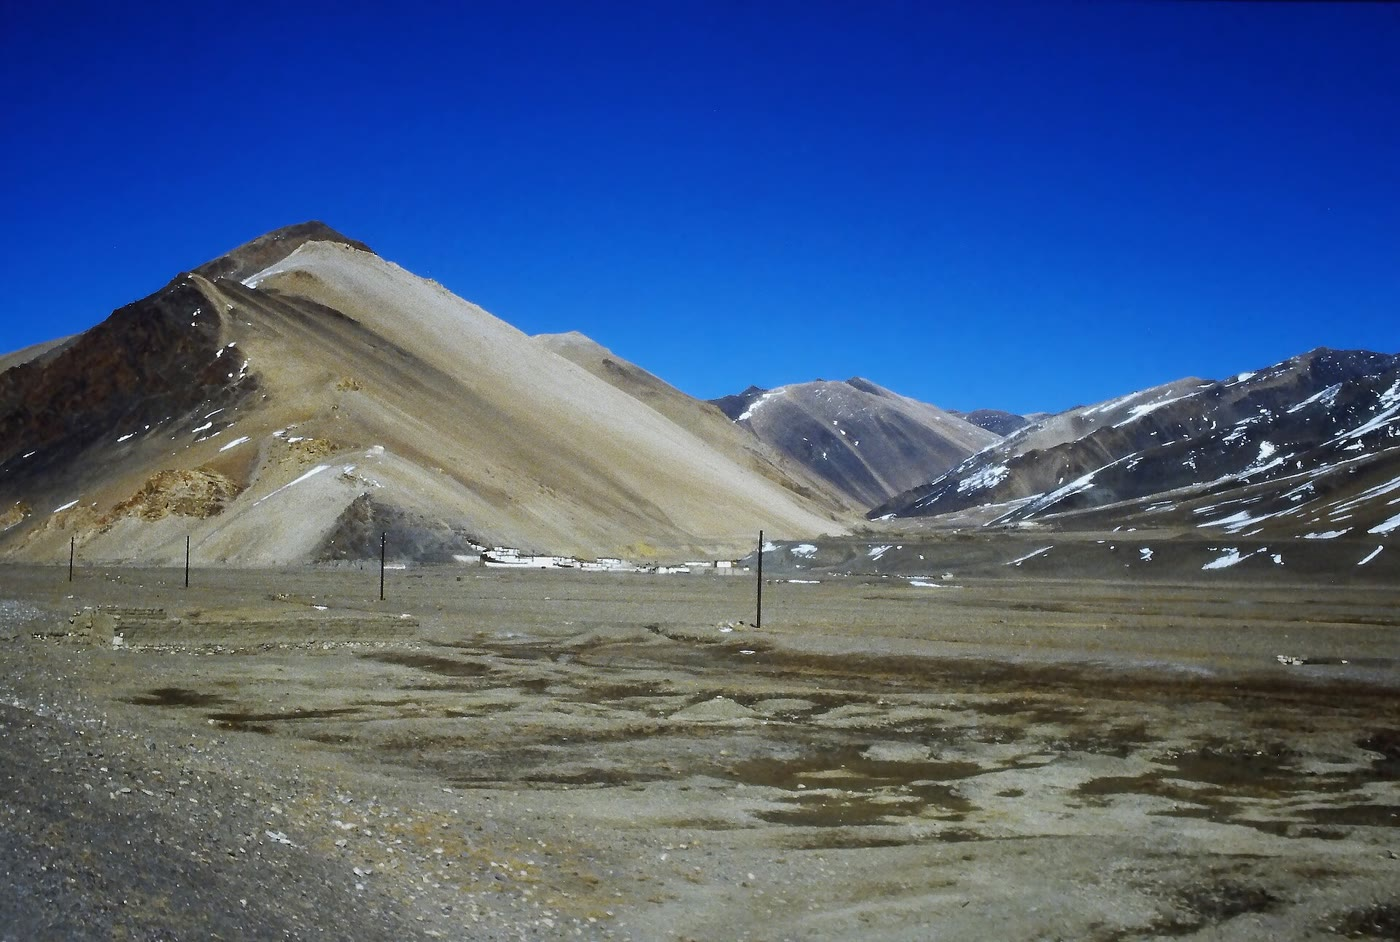
\includegraphics[width=0.66\linewidth]{images/book4/b2-14-tibet-plateau.jpg}
\par\smallskip{\small Le plateau tibétain entre le Népal et Shigatsé~:
un plancher plat de gravier et de maigres pâturages, avec un village,
entre des montagnes nues couvertes d'éboulis, le tout à plus de quatre
kilomètres d'altitude. Photographie Jan Kranendonk, 1987, CC BY-SA 4.0.}
\end{omfigure}
% ledger: data:b4-etopo-tibet

\subsection{Le poids d'un plateau}

Un plateau pèse sur son environnement. À toute profondeur jusqu'à la base de sa racine, une colonne
sous le plateau subit une pression plus forte qu'une colonne sous les plaines voisines~; seule
à la profondeur de compensation elles sont égales. La colonne haute pousse vers l'extérieur.

\begin{proposition}[Énergie potentielle excédentaire d'un plateau]\label{prop:b2:himalaya-andes:gpe}
Dans les hypothèses de la \cref{prop:b2:himalaya-andes:airy}, avec la pesanteur $g$,
l'intégrale de la surpression lithostatique de la colonne du plateau sur la colonne normale,
du sommet du plateau à la profondeur de compensation à la base de sa racine $r$, vaut
\[
  \Delta F = \rho_c g h \left(H + \frac{h}{2} + \frac{r}{2}\right) .
\]
Il s'agit de l'énergie potentielle gravitaire excédentaire de la colonne
du plateau par unité d'aire, et de la force par unité de longueur
du bord du plateau avec laquelle celui-ci pousse son environnement.
\end{proposition}

\begin{proof}
Mesurons la profondeur $z$ vers le bas à partir du niveau de
la mer. Dans la colonne du plateau, la pression vaut $p_1 =
\rho_c g (z + h)$ de $z = -h$ à $L = H + r$. Dans la colonne normale, elle est nulle au-dessus du niveau de
la mer, vaut $\rho_c g z$ dans la croûte, et $\rho_c g H + \rho_m g (z - H)$ en dessous. La différence $p_1
- p_0$ croît de 0 en $z = -h$ à $\rho_c g h$ au niveau de la mer~; elle garde cette valeur à travers
la croûte normale, où les deux colonnes sont de la croûte~; sous $z = H$, elle décroît linéairement,
de $(\rho_m - \rho_c) g$ par mètre, et s'annule en $L$ puisque $(\rho_m - \rho_c) r = \rho_c
h$. L'intégrale est l'aire de ce trapèze~: $\rho_c g h\,(h/2 + H + r/2)$. Le travail des pressions lorsque les deux colonnes
échangent de la matière latéralement est cette intégrale, ce qui explique qu'elle mesure à la fois l'énergie et la poussée.
\end{proof}

\begin{omfigure}
\centering
% figdata/bachelor-2/plateaus.py part pressure (h = 4.8 km, H = 35 km, 2700 and 3300 kg/m3)
\begin{tikzpicture}
\begin{axis}[width=0.62\linewidth, height=5.6cm, y dir=reverse, xmin=0, xmax=160, ymin=-12,
  ymax=60, xlabel={surpression $p_1 - p_0$ (\unit{MPa})}, ylabel={profondeur sous le niveau de la mer
  (\unit{km})}, tick label style={font=\scriptsize}, label style={font=\small},
  xtick pos=bottom, ytick pos=left, clip=false]
\addplot[fill=omThm!20, draw=omThm, line width=1pt] table[x expr=\thisrow{p_high_MPa}-\thisrow{p_ref_MPa}, y=z_km] {figdata/out/bachelor-2-plateaus-pressure.dat} \closedcycle;
\draw[dashed] (axis cs:0,0) -- (axis cs:160,0);
\draw[dashed] (axis cs:0,35) -- (axis cs:160,35);
\draw[dashed] (axis cs:0,56.6) -- (axis cs:160,56.6);
\node[font=\scriptsize, anchor=north east] at (axis cs:160,0) {niveau de la mer};
\node[font=\scriptsize, anchor=north east] at (axis cs:160,35) {Moho normal, $H$};
\node[font=\scriptsize, anchor=south east] at (axis cs:160,56.6) {base de la racine, $H + r$};
\node[font=\scriptsize, anchor=west] at (axis cs:100,-8.4) {sommet du plateau, $-h$};
\node[font=\scriptsize, align=center] at (axis cs:60,20) {aire $= \Delta F$\\$\approx\qty{6.1e12}{N.m^{-1}}$};
\end{axis}
\end{tikzpicture}
\par\smallskip{\small Surpression lithostatique d'une colonne de plateau par rapport à
une colonne normale, pour $h = \qty{4.8}{km}$, $H = \qty{35}{km}$ et des masses volumiques
de 2700 et \qty{3300}{kg.m^{-3}}~: elle croît à travers le plateau, reste à
$\rho_c g h = \qty{127}{MPa}$ dans la croûte normale, et tombe à zéro à la base de la racine. L'aire
grisée est l'énergie potentielle excédentaire de la \cref{prop:b2:himalaya-andes:gpe}.}
\end{omfigure}
% values (plateaus.py): tibet_gpe 6.12179e12 N/m for h = 4.8

Pour le Tibet, $r = 4.5 \times 4.8 = \qty{21.6}{km}$ et $\Delta F = 2700 \times 9.8 \times 4800
\times (35000 + 2400 + 10800) \approx \qty{6.1e12}{N.m^{-1}}$. Étalée sur une lithosphère de \qty{100}{km}
d'épaisseur, cela représente une contrainte excédentaire moyenne d'environ \qty{60}{MPa}, de l'ordre des
contraintes qui brisent les roches. Un plateau si lourd ne peut plus simplement s'élever~: il tend à s'étaler.

\begin{definition}[Effondrement gravitaire]\label{def:b2:himalaya-andes:collapse}
L'\emph{effondrement gravitaire}\index{effondrement gravitaire (d'un orogène)}
d'un \omterm{def:b2:alpine-orogen:orogen}{orogène} est l'étalement de sa croûte épaissie sous son propre poids, par
extension des régions élevées et écoulement vers l'extérieur ou chevauchement aux
bords, sous l'effet de l'énergie potentielle excédentaire des colonnes épaissies.
\end{definition}

Le Tibet s'étire alors que l'Inde le pousse encore. Dans le sud du Tibet, des rifts nord--sud découpent
le plateau et accommodent une extension est--ouest~: environ $9 \pm \qty{2}{mm}$ par an au total
entre \ang{81} et \ang{92}~E, et $1.3 \pm \qty{0.3}{mm}$ par an sur le seul rift de Yadong--Gulu~; au
nord du Népal, les stations GPS montrent que le plateau méridional s'étire d'environ \num{12e-9} par
an. Les séismes racontent la même histoire~: chevauchements et \omterm{def:b2:himalaya-andes:thickening}{épaississement crustal} dominent les
terrains bas qui entourent le plateau, décrochements et failles normales à son intérieur. La raison
de cette extension fait débat. Sur le plateau oriental, l'extension a été interprétée comme un \omterm{def:b2:himalaya-andes:collapse}{effondrement
gravitaire} piloté par le poids du plateau~; au sud, d'autres la relient à la courbure de l'arc
himalayen, le long duquel les chevauchements divergent, ou au glissement de l'Inde sous le plateau.
% ledger: wang21:rifts, ader12:extension

\subsection{S'échapper latéralement}

\begin{definition}[Extrusion latérale]\label{def:b2:himalaya-andes:extrusion}
L'\emph{extrusion latérale}\index{extrusion latérale} (tectonique d'échappement) est l'expulsion
de blocs de croûte ou de lithosphère sur le côté, hors d'une zone de collision, le long de grands
décrochements à peu près perpendiculaires à la direction de convergence, vers un bord libre.
\end{definition}

À l'est du Tibet, l'Asie n'est pas seulement raccourcie~; elle est repoussée sur le côté. De longs décrochements
senestres, dont la faille de la Rivière Rouge et celle de l'Altyn Tagh, sont interprétés comme ayant
guidé l'échappement vers l'est et le sud-est de grands blocs~: d'abord le bloc de la Sonde en Asie du
Sud-Est, puis le Tibet et la Chine du Sud, tandis que des rifts et de jeunes bassins océaniques s'ouvraient
à leurs extrémités lointaines. Des expériences où un poinçon rigide était enfoncé dans une couche de pâte
à modeler ont produit de telles failles~; des modèles traitant l'Asie comme une feuille visqueuse continue
produisaient au contraire un épaississement diffus, sans grande faille. Le GPS confirme le mouvement
des blocs~: par rapport à la Sibérie stable, le bassin du Tarim se déplace à peu près vers le nord à environ
\qty{14}{mm} par an, et la Chine du Sud vers l'est-sud-est à environ \qty{8}{mm} par an. Quelle part de
l'avancée de l'Inde a été absorbée par l'épaississement, et quelle part par l'extrusion, reste débattu.
% ledger: jiao23:extrusion

\section{Les Andes}\label{sec:b2:himalaya-andes:andes}

La plaque de Nazca plonge sous l'Amérique du Sud à environ \qty{72}{mm} par an près de \ang{20}~S,
vers l'est-nord-est, d'après les vitesses angulaires de NNR-MORVEL56. Aucun continent n'est
arrivé, et pourtant les Andes centrales portent le deuxième plateau le plus haut de la Terre.
% ledger: nnr56:poles
% values (plateaus.py): v_nazca_southamerica 72.52 mm/yr, azimuth 74.5

D'ouest en est, entre environ \ang{15} et \ang{27}~S, on distingue cinq zones~: l'\emph{avant-arc}~;
la \emph{Cordillère occidentale}, l'arc volcanique~; le haut plateau, l'\emph{Altiplano}
au nord et la \emph{Puna} au sud~; la \emph{Cordillère orientale}~; et la \omterm{def:b2:alpine-orogen:ftb}{chaîne plissée
et chevauchante} de \omterm{def:b2:alpine-orogen:skin}{tectonique de couverture} de la \emph{zone subandine}, qui se prolonge
dans la plaine du Chaco. Le profil ci-dessus les traverse à \ang{20}~S~: depuis la fosse, dont
le point le plus profond se trouve à \qty{7.7}{km} sous le niveau de la mer à \ang{71.4}~O,
la surface remonte de plus de \qty{11}{km} en environ \qty{240}{km} jusqu'au bord du
plateau, à \ang{69.1}~O~; le plateau reste au-dessus de \qty{3000}{m} sur \qty{440}{km}, avec une
moyenne de \qty{3760}{m}. L'altitude moyenne est de \qty{3.7}{km} dans l'Altiplano et de
\qty{4.4}{km} dans la Puna. Au nord de \ang{23}~S, le Moho est généralement plus profond que
\qty{60}{km}~; sous l'Altiplano central, la croûte mesure de 59 à \qty{64}{km} d'épaisseur.
% ledger: gerbault05:andes, gerbault05:moho, data:b4-etopo-andes

\begin{omfigure}
\centering
\begin{tikzpicture}[x=0.56cm, y=0.38cm, font=\scriptsize]
% mantle background
\fill[gray!12] (0,-2.6) -- (5,-3.6) -- (8,-5.6) -- (10,-9.1) -- (12,-12.6) -- (13.2,-14.6) -- (26,-14.6)
  -- (26,-4.5) -- (20,-4.7) -- (17.5,-6.0) -- (15,-7.3) -- (11,-7.0) -- (9.5,-6.2) -- (8,-4) -- (5,-2)
  -- (0,-1) -- cycle;
% ocean water
\fill[blue!8] (0,0) -- (6.33,0) -- (5,-2) -- (0,-1) -- cycle;
% Nazca slab
\fill[gray!45] (0,-1) -- (5,-2) -- (8,-4) -- (10,-7.5) -- (12,-11) -- (14,-14.5) -- (13.2,-14.6)
  -- (12,-12.6) -- (10,-9.1) -- (8,-5.6) -- (5,-3.6) -- (0,-2.6) -- cycle;
% South American crust
\fill[orange!22] (5,-2) -- (8,1) -- (9,1.9) -- (10.2,2.0) -- (11,2.0) -- (15,2.0) -- (15.6,2.6) -- (16.8,2.4)
  -- (17.5,1.6) -- (20,0.6) -- (20.6,0.4) -- (26,0.3) -- (26,-4.5) -- (20,-4.7) -- (17.5,-6.0) -- (15,-7.3)
  -- (11,-7.0) -- (9.5,-6.2) -- (8,-4) -- cycle;
% Altiplano basin fill
\fill[yellow!45] (11,2.0) -- (15,2.0) -- (14.6,1.0) -- (11.4,1.0) -- cycle;
% surface line
\draw[line width=0.5pt] (0,-1) -- (5,-2) -- (8,1) -- (9,1.9) -- (10.2,2.0) -- (11,2.0) -- (15,2.0) -- (15.6,2.6)
  -- (16.8,2.4) -- (17.5,1.6) -- (20,0.6) -- (20.6,0.4) -- (26,0.3);
% arc volcanoes
\fill[red!60!black] (8.8,1.75) -- (9.2,2.9) -- (9.6,1.95) -- cycle;
\fill[red!60!black] (9.8,1.95) -- (10.2,2.8) -- (10.6,2.0) -- cycle;
\draw[red!60!black, decorate, decoration={snake, amplitude=0.6pt, segment length=4pt}] (10.8,-8.0) -- (9.9,1.6);
% Subandean decollement and splays
\draw[thick] (16.0,-1.2) -- (20.55,0.42);
\draw (17.4,-0.7) -- (17.85,1.45);
\draw (18.4,-0.35) -- (18.8,1.08);
\draw (19.4,0.0) -- (19.7,0.72);
% Moho
\draw[dashed] (8,-4) -- (9.5,-6.2) -- (11,-7.0) -- (15,-7.3) -- (17.5,-6.0) -- (20,-4.7) -- (26,-4.5);
% labels
\node at (2.6,-0.5) {Pacifique};
\node at (2.4,-2.2) {plaque de Nazca};
\draw[-{Latex[length=1.6mm]}] (1.6,-2.8) -- (3.2,-3.0);
\node[anchor=south] (tr) at (4.3,0.9) {fosse};
\draw[->] (tr.south) -- (5,-1.8);
\node[anchor=south east] at (7.6,1.0) {avant-arc};
\node[anchor=south, align=center] at (9.7,3.0) {Cordillère\\occidentale (arc)};
\node[anchor=south] at (13,2.1) {Altiplano};
\node[anchor=south, align=center] at (16.4,2.7) {Cordillère\\orientale};
\node[anchor=south west] at (18.6,1.3) {subandine};
\node[anchor=south] at (23.5,0.4) {plaine du Chaco};
\node at (13,-3.2) {croûte épaisse};
\node at (23.2,-2.0) {bouclier brésilien};
\node[anchor=north] at (23.2,-4.6) {Moho};
\node at (14.2,-9.6) {coin mantellique};
\node at (21,-10) {manteau};
\node[rotate=-50] at (12.75,-12.9) {plaque};
\draw[-{Latex[length=2mm]}] (1.2,4.6) -- (0.2,4.6);
\node[anchor=south] at (0.7,4.6) {O};
\draw[-{Latex[length=2mm]}] (24.8,4.6) -- (25.8,4.6);
\node[anchor=south] at (25.3,4.6) {E};
\end{tikzpicture}
\par\smallskip{\small Coupe schématique à travers les Andes centrales, vers \ang{20}~S (sans échelle).
La plaque de Nazca s'enfonce sous l'avant-arc~; le \omterm{def:b2:magma-emplacement:magma}{magma} monte du coin mantellique (ligne ondulée)
jusqu'à l'arc de la Cordillère occidentale~; l'Altiplano, avec son épais remplissage de bassin, se
place entre les deux cordillères, au-dessus d'une croûte d'environ \qty{60}{km} d'épaisseur~; la
chaîne subandine, plissée et de \omterm{def:b2:alpine-orogen:skin}{tectonique de couverture}, chevauche vers l'est le bouclier brésilien.}
\end{omfigure}
% ledger: gerbault05:andes, gerbault05:moho

\subsection{Comment la croûte s'est épaissie}

D'où vient la croûte supplémentaire de l'Altiplano~? La première piste est le raccourcissement~:
on comprime une bande de croûte, elle s'épaissit en conservant sa section transversale.

\begin{proposition}[Épaississement par raccourcissement]\label{prop:b2:himalaya-andes:shortening}
Soit une croûte d'épaisseur uniforme $H$, raccourcie sans gain ni perte de roche, en
une croûte d'épaisseur $T$ sur une largeur $W$, la section restant parallèle au
raccourcissement. Sa largeur initiale était $W_0 = W T/H$, et le raccourcissement vaut
\[
  S = W_0 - W = W\,\frac{T - H}{H} .
\]
\end{proposition}

\begin{proof}
L'aire de section de la croûte se conserve, comme dans le bilan d'aire de la
\cref{prop:b2:alpine-orogen:balance}~: $W_0 H = W T$. D'où $W_0 = WT/H$ et $S = W_0 - W =
W(T - H)/H$.
\end{proof}

À \ang{20}~S, le plateau a environ \qty{440}{km} de large~; si sa croûte, d'environ \qty{60}{km} d'épaisseur,
valait autrefois \qty{35}{km}, le raccourcissement nécessaire est $440 \times 25/35 \approx \qty{314}{km}$.
Des \omterm{def:b2:alpine-orogen:balanced}{coupes équilibrées} près de 16--\ang{21}~S trouvent environ \qty{50}{km} de raccourcissement dans
l'Altiplano et plus de \qty{200}{km} dans la zone subandine depuis l'Oligocène. Les volumes de croûte calculés
à partir du raccourcissement restent d'environ \qty{20}{\percent} inférieurs à ceux calculés à partir de
la profondeur du Moho. Une part de l'écart peut tenir à des hypothèses erronées, sur l'épaisseur initiale
ou sur la nature du Moho sismique~; une autre part peut venir de croûte ajoutée par d'autres voies. Une
compilation proche de \ang{21}~S attribue au raccourcissement tectonique au moins \qty{55}{\percent} de la
racine, à l'hydratation du coin mantellique de l'avant-arc jusqu'à \qty{20}{\percent}, et à l'apport magmatique
et à l'érosion tectonique seulement environ \qty{5}{\percent}. La roche peut aussi se déplacer à l'intérieur
de la chaîne~: les différences d'épaisseur crustale créent des différences d'énergie potentielle, comme
au Tibet, et celles-ci peuvent conduire la croûte inférieure chaude à s'écouler de l'épais vers le mince.
% ledger: gerbault05:andes, gerbault05:volume, gerbault05:moho, data:b4-etopo-andes

\begin{omfigure}
\centering
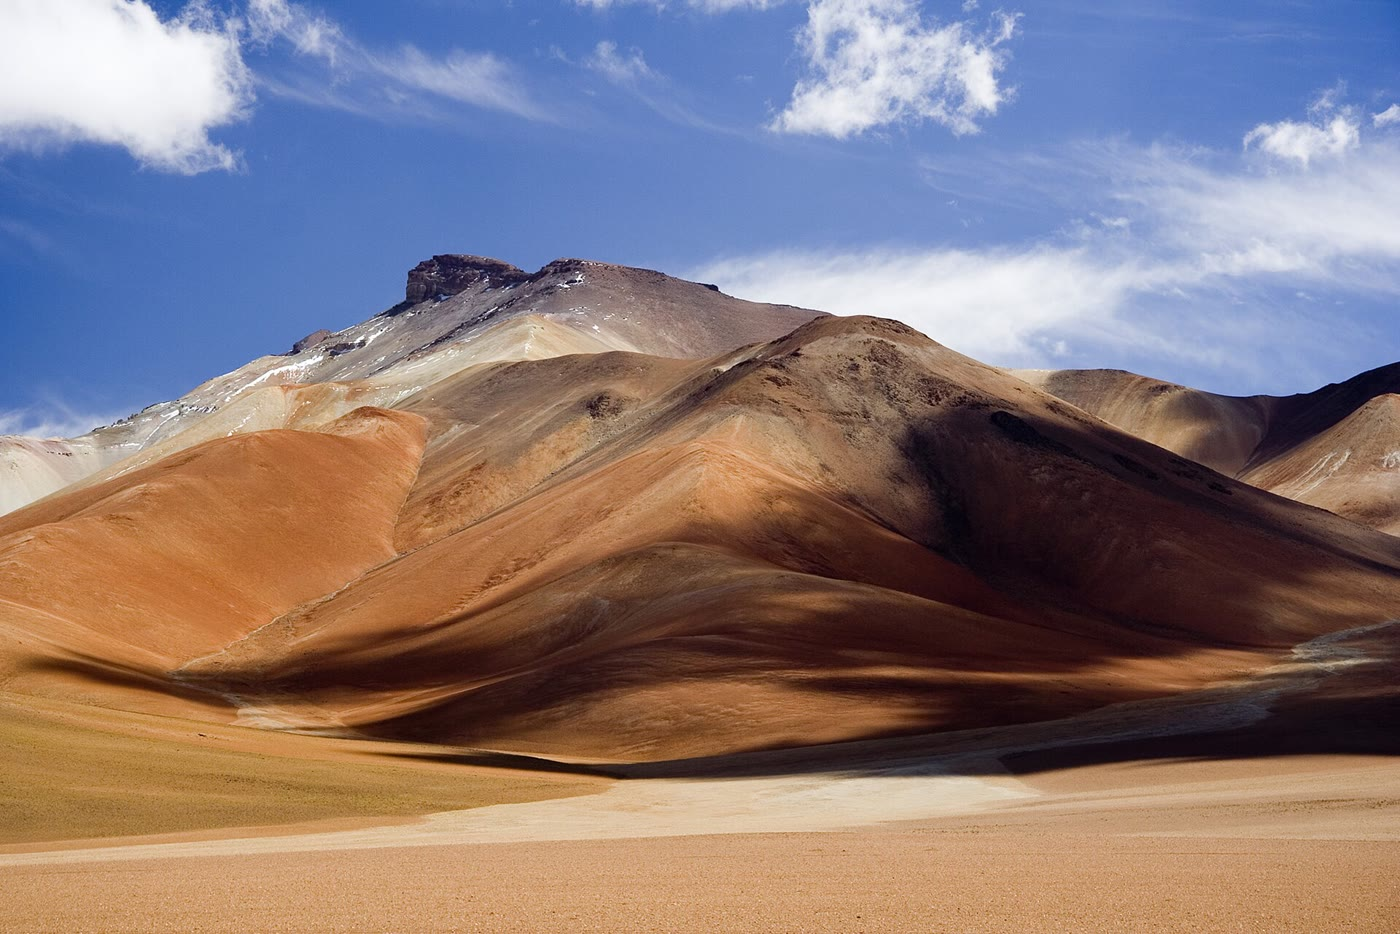
\includegraphics[width=0.66\linewidth]{images/book4/b2-14-altiplano.jpg}
\par\smallskip{\small L'Altiplano bolivien~: une plaine de sable et de gravier au pied de collines
nues, colorées en rouge, ocre et gris par leurs roches. Photographie Luca Galuzzi, 2006, CC BY-SA 2.5.}
\end{omfigure}
% ledger: gerbault05:andes

\subsection{Plaques plates et racines perdues}

L'angle de la plaque plongeante n'est pas fixe, et il compte en surface.

\begin{definition}[Subduction plane]\label{def:b2:himalaya-andes:flat-slab}
La \emph{subduction plane}\index{subduction plane} est une subduction dans laquelle
la plaque plongeante, après sa première descente, court presque horizontalement
sous la plaque chevauchante pendant des centaines de kilomètres avant de replonger.
\end{definition}

Dans les Andes, deux segments de la plaque de Nazca sont aujourd'hui plats~: le segment péruvien, plat
depuis environ \qty{15}{Ma}, et le segment pampéen, depuis environ \qty{18}{Ma}. Au-dessus d'eux,
aucun volcan n'est actif. Quand la plaque pampéenne s'est aplatie, l'arc s'est déplacé vers l'intérieur
des terres et a émis moins de lave~; au-dessus des segments plats, il s'est tu. L'écart arc--fosse
du volume de première année explique ce déplacement vers l'intérieur~: plus la plaque est douce
sous l'arc, plus loin de la fosse elle atteint la profondeur à laquelle le coin fond~; et une plaque
qui reste plate au-dessus de cette profondeur ne laisse aucun coin de manteau chaud pour fondre.
% ledger: gauthier24:flat

\begin{definition}[Délamination lithosphérique]\label{def:b2:himalaya-andes:delamination}
La \emph{délamination lithosphérique}\index{délamination lithosphérique} est le détachement et
l'enfoncement dans l'asthénosphère de la partie basse d'une lithosphère épaissie, de son manteau
lithosphérique et parfois d'une croûte inférieure dense, remplacés par de l'asthénosphère chaude.
\end{definition}

On a proposé une délamination sous la Puna méridionale, entre \ang{24} et \ang{27}~S, il y
a environ 2 à \qty{3}{Ma}, là où des laves mafiques jeunes ont jailli~; et le long du plateau,
les variations d'épaisseur crustale et d'altitude ont été reliées à un manteau lithosphérique
déjà retiré sous l'Altiplano méridional, et pas encore complètement sous l'Altiplano
central. Perdre un couvercle mantellique dense rend la colonne restante plus légère~: la
surface s'élève sans aucun raccourcissement supplémentaire. La Puna se dresse environ \qty{1}{km}
plus haut que l'Altiplano sur une croûte d'environ \qty{11}{km} plus mince, un contraste
qui exige soit une croûte de la Puna plus légère, soit un manteau plus léger sous elle.
% ledger: gerbault05:delamination, gerbault05:moho

\section{Deux chaînes comparées}\label{sec:b2:himalaya-andes:compared}

De loin, les deux plateaux se ressemblent et diffèrent sur
presque tout le reste, comme le rassemble le tableau ci-dessous.

\begin{omfigure}
\centering\small
\begin{tabular}{>{\raggedright\arraybackslash}p{0.2\linewidth}|>{\raggedright\arraybackslash}p{0.34\linewidth}|>{\raggedright\arraybackslash}p{0.34\linewidth}}
 & Himalaya et Tibet & Andes centrales \\ \hline
moteur & continent contre continent après la fermeture de l'océan & plaque océanique qui plonge sous un continent \\
axe & suture à \omterm{def:b2:alpine-orogen:ophiolite}{ophiolites} & arc volcanique au-dessus de la plaque plongeante \\
magmatisme & fusions crustales~: \omterm{def:b2:crustal-melting:leucogranite}{leucogranites} & andésites d'arc~; laves mafiques là où la lithosphère a été perdue \\
convergence & environ \qty{45}{mm} par an, dont la moitié absorbée par la chaîne & environ \qty{72}{mm} par an, consommés pour l'essentiel par la subduction \\
grands séismes & sur le MHT, Assam 1950, $M_w \approx 8.5$ & sur l'interface de subduction, Chili 1960, $M_w$ 9.5 \\
plateau & altitude moyenne \qty{4.8}{km} sur \qty{1180}{km}~; croûte 70--\qty{75}{km} & altitude moyenne \qty{3.8}{km} sur \qty{440}{km}~; croûte d'environ \qty{60}{km} \\
tectonique des plateaux & extension est--ouest, extrusion & raccourcissement sur les flancs~; délamination proposée \\
avant-pays & avant-fosse indo-gangétique et \omterm{def:b2:alpine-orogen:foreland}{molasse} des Siwaliks & zone subandine et plaine du Chaco \\
\end{tabular}
\par\smallskip{\small Les deux chaînes côte à côte~; les sources sont citées dans les
sections ci-dessus, et le séisme du Chili est le plus fort enregistré depuis 1900.}
\end{omfigure}
% ledger: lave00:setting, lave00:siwaliks, weinberg16:himalaya, ader12:mht, ader12:quakes, usgs:largest, gerbault05:andes, gerbault05:moho, gerbault05:delamination, nnr56:poles, data:b4-etopo-tibet, data:b4-etopo-andes, cattin01:crust, wang21:rifts, jiao23:extrusion

La différence la plus profonde tient à ce qui s'enfonce. Dans les Andes, la plaque océanique continue
de plonger, et l'essentiel de la convergence, environ \qty{72}{mm} par an, est consommé à la fosse~;
raccourcir la plaque supérieure de \qty{310}{km} sur environ \qty{30}{Ma} n'en absorberait qu'environ
\qty{10}{mm} par an. En revanche, dans l'Himalaya, rien de léger ne peut plonger longtemps, si bien
que la convergence est dépensée à empiler, à épaissir et à repousser l'Asie sur le côté. Les deux
chaînes produisent des plateaux parce qu'une croûte épaisse est une croûte haute~; les deux plateaux
cessent de s'élever lorsque leur propre poids équilibre la poussée à leurs bords, puis ils s'étalent.
% ledger: nnr56:poles, gerbault05:andes, ader12:mht, jiao23:extrusion

\section{Quelle altitude une montagne peut-elle atteindre~?}\label{sec:b2:himalaya-andes:heights}

Le sommet le plus élevé, l'Everest, culmine à \qty{8848.86}{m} au-dessus du niveau de la mer, selon le relevé
conjoint annoncé en 2020. Pourquoi pas vingt kilomètres~? Une borne grossière vient de la résistance des roches.

\begin{proposition}[Une limite de hauteur fixée par la résistance des roches]\label{prop:b2:himalaya-andes:height}
Une colonne de roche de masse volumique $\rho$, dressée à une hauteur $h$ au-dessus de son environnement,
sans appui latéral au-dessus de leur niveau, porte à sa base une contrainte verticale $\rho g h$ et, sur
ses faces libres, une contrainte horizontale nulle~; la contrainte différentielle vaut donc $\rho g h$. Si
la roche rompt à la contrainte différentielle $\sigma_d$, la colonne ne tient que si $h < \sigma_d/(\rho
g)$.
\end{proposition}

\begin{proof}
À la base de la colonne, la contrainte verticale est le poids de la roche située au-dessus, par
unité d'aire, soit $\rho g h$. Les faces sont libres, donc la contrainte horizontale y est nulle.
La contrainte différentielle est la différence entre la plus grande et la plus petite contrainte
principale, ici $\rho g h - 0$. La rupture n'est évitée que si elle reste inférieure à $\sigma_d$.
\end{proof}

Une vraie montagne a des flancs en pente qui retiennent son cœur, de sorte
que la contrainte qui s'exerce sous elle est plus faible~; comme ordre de
grandeur, prenons la moitié, $\rho g h/2$. Pour l'Everest, $2700 \times 9.8
\times 8849/2 \approx \qty{117}{MPa}$. La loi de Byerlee du volume de première année donne la résistance au
frottement d'une roche sur une faille sous une contrainte normale de \qty{200}{MPa}~: $50 + 0.6 \times 200 =
\qty{170}{MPa}$, du même ordre. Une montagne trois fois plus haute chargerait sa base bien au-delà de ce que
la roche peut supporter~; elle céderait et s'étalerait. Sur Terre, les sommets de huit à neuf kilomètres sont
proches de la limite, et un plateau, qui s'étale bien avant que ses sommets ne cèdent, s'arrête vers cinq.
% ledger: tht:everest, byerlee:1975

\section*{Exercices}\label{sec:b2:himalaya-andes:exercises}

Données~: $g = \qty{9.8}{m.s^{-2}}$~; masses volumiques de la croûte et du manteau
\qty{2700}{kg.m^{-3}} et \qty{3300}{kg.m^{-3}} sauf indication contraire~; croûte normale $H =
\qty{35}{km}$.

\begin{exercise}[$\star$]\label{exo:b2:himalaya-andes:1}
Un plateau se dresse à une altitude moyenne de \qty{3.0}{km}. En utilisant la
\cref{prop:b2:himalaya-andes:airy}, calculer (a) sa racine d'Airy, (b) son épaisseur
crustale. (c) De combien \qty{10}{km} de croûte supplémentaire le relèveraient-ils~?
\end{exercise}

\begin{exercise}[$\star$]\label{exo:b2:himalaya-andes:2}
Un profil de l'Himalaya du Népal va de la plaine du Gange au plateau tibétain. (a)
Énumérer, dans l'ordre, les unités traversées et les failles qui les séparent. (b)
Quelle faille est une faille normale~? (c) Comment le degré de \omterm{def:b2:metamorphic-facies:metamorphism}{métamorphisme}
change-t-il vers le nord jusqu'à la séquence du Grand Himalaya, puis au-dessus d'elle~?
\end{exercise}

\begin{exercise}[$\star$]\label{exo:b2:himalaya-andes:3}
Au centre du Népal, une terrasse de rivière abandonnée il y a \qty{9.2}{ka} a été raccourcie
de \qty{196.5}{m} à travers les plis du chevauchement frontal principal. (a) Calculer le taux de
raccourcissement moyen, en millimètres par an. (b) Le comparer à la convergence GPS à travers
la chaîne, \qty{17.8}{mm} par an. (c) Que dit cet accord des failles situées au nord du MFT~?
\end{exercise}

\begin{exercise}[$\star$]\label{exo:b2:himalaya-andes:4}
Classer chaque observation en \omterm{def:b2:himalaya-andes:types}{orogène de collision}, en \omterm{def:b2:himalaya-andes:types}{orogène de type andin} ou dans les deux cas~:
(a) une suture bordée d'\omterm{def:b2:alpine-orogen:ophiolite}{ophiolites}~; (b) une ligne de volcans andésitiques actifs~; (c) des \omterm{def:b2:crustal-melting:leucogranite}{leucogranites}
fondus à partir de la croûte~; (d) une fosse océanique profonde le long du front~; (e) un
\omterm{def:b2:alpine-orogen:foreland}{bassin d'avant-pays} à \omterm{def:b2:alpine-orogen:foreland}{molasse}~; (f) de grands séismes sur une faille à faible pendage sous la chaîne.
\end{exercise}

\begin{exercise}[$\star\star$]\label{exo:b2:himalaya-andes:5}
L'Inde se déplace à \qty{45}{mm} par an par rapport à l'Eurasie à travers l'Himalaya~; à
travers le Népal, la chaîne elle-même absorbe \qty{17.8}{mm} par an à l'est et \qty{20.5}{mm}
par an à l'ouest. (a) Quelle fraction de la convergence la chaîne prend-elle dans chaque cas~?
(b) Où va le reste~? (c) Sur \qty{10}{Ma}, quel raccourcissement représente le reliquat~?
\end{exercise}

\begin{exercise}[$\star\star$]\label{exo:b2:himalaya-andes:6}
(a) En utilisant la \cref{prop:b2:himalaya-andes:gpe}, calculer l'énergie potentielle excédentaire de
l'Altiplano, d'altitude moyenne \qty{3.7}{km}. (b) La comparer à celle du Tibet, à \qty{4.8}{km}. (c)
Montrer que pour un plateau mince, $h \ll H$, $\Delta F$ croît proportionnellement à $h$, et que pour
un plateau épais il croît plus vite~: qu'est-ce que cela implique pour la croissance d'un plateau~?
\end{exercise}

\begin{exercise}[$\star\star$]\label{exo:b2:himalaya-andes:7}
(a) Calculer $\rho g h/2$ sous l'Everest, haut de \qty{8848.86}{m}, avec $\rho =
\qty{2700}{kg.m^{-3}}$. (b) Selon la loi de Byerlee, $\tau = 0.85\,\sigma_n$ en dessous de \qty{200}{MPa} de
contrainte normale et $\tau = \qty{50}{MPa} + 0.6\,\sigma_n$ au-dessus~; calculer $\tau$ pour $\sigma_n =
100$ et \qty{200}{MPa}. (c) Quelle hauteur une résistance de
\qty{170}{MPa} permettrait-elle, avec la même règle d'ordre de grandeur~?
\end{exercise}

\begin{exercise}[$\star\star$]\label{exo:b2:himalaya-andes:8}
Les rifts du Tibet méridional absorbent $9 \pm \qty{2}{mm}$ par an d'extension est--ouest entre \ang{81}
et \ang{92}~E. (a) Quelle largeur représente cette bande à \ang{30}~N, avec \qty{111.19}{km} par
degré sur un méridien~? (b) Calculer le taux d'extension moyen, par an et par seconde, avec son
intervalle. (c) Le comparer aux $(12.4 \pm 4.7) \times 10^{-9}$ par an trouvés par GPS au nord du Népal.
\end{exercise}

\begin{exercise}[$\star\star$]\label{exo:b2:himalaya-andes:9}
Le chevauchement principal de l'Himalaya, bloqué sous le Népal, accumule un déficit de moment
de \qty{6.6e19}{N.m} par an~; les séismes des 500 dernières années n'en ont libéré que
\qty{0.9e19}{N.m} par an. (a) Quelle fraction du déficit ont-ils libérée~? (b) Avec $M_0 =
10^{1.5 M_w + 9.1}$\,\unit{N.m}, calculer le moment d'un séisme de magnitude $M_w$
8.5. (c) À quelle fréquence faudrait-il de tels séismes pour compenser le déficit~?
\end{exercise}

\begin{exercise}[$\star\star\star$]\label{exo:b2:himalaya-andes:10}
La Puna se dresse \qty{0.7}{km} plus haut que l'Altiplano (4.4 contre \qty{3.7}{km}) sur une croûte
\qty{11}{km} plus mince. Prendre la croûte de l'Altiplano épaisse de \qty{61.5}{km} et de masse volumique
\qty{2800}{kg.m^{-3}}, et un manteau de \qty{3300}{kg.m^{-3}} sous les deux. (a) Écrire l'égalité
des masses des deux colonnes au-dessus d'une profondeur de compensation commune. (b) Trouver la masse
volumique que doit avoir la croûte de la Puna si la seule croûte compense la différence. (c) Comparer
avec les 150 à \qty{200}{kg.m^{-3}} cités, et dire ce qui d'autre pourrait expliquer le contraste~?
\end{exercise}

\begin{exercise}[$\star\star\star$]\label{exo:b2:himalaya-andes:11}
Le front volcanique se trouve là où le sommet de la plaque plongeante est à \qty{105}{km} de profondeur.
(a) Pour une plaque à pendage uniforme de \ang{30}, calculer l'écart arc--fosse avec la formule
du volume de première année. (b) La plaque plonge désormais à \ang{30} jusqu'à \qty{90}{km}, puis
à seulement \ang{4}~: calculer le nouvel écart et le déplacement vers l'intérieur de l'arc. (c)
Que devient l'arc si la plaque s'aplatit à \qty{95}{km} de profondeur et y reste sur \qty{300}{km}~?
\end{exercise}

\begin{exercise}[$\star\star\star$]\label{exo:b2:himalaya-andes:12}
L'érosion enlève environ \qty{300}{km^3} de roche par kilomètre d'Himalaya et par million
d'années. L'Inde apporte une croûte épaisse de \qty{37.5}{km} à \qty{21}{mm} par an. (a)
Quelle quantité de croûte, par kilomètre de chaîne et par million d'années, entre dans la
ceinture~? (b) Quelle fraction l'érosion enlève-t-elle~? (c) Où peut se trouver le reste~?
\end{exercise}

\begin{problem}[{Problème du week-end --- deux plateaux}]\label{pb:b2:himalaya-andes:1}
Les profils par bandes de ce chapitre donnent l'altitude moyenne des nœuds à travers le Tibet
(\qtyrange{86}{90}{\degree}~E) et à travers les Andes centrales (\qtyrange{19}{21}{\degree}~S). Échantillonnés
tous les \ang{1.5} de latitude et tous les degrés de longitude, arrondis à \qty{10}{m}, ils se
lisent comme suit. Sauf indication contraire, $g = \qty{9.8}{m.s^{-2}}$, $\rho_c = \qty{2700}{kg.m^{-3}}$,
$\rho_m = \qty{3300}{kg.m^{-3}}$ et la croûte normale a pour épaisseur $H = \qty{35}{km}$.

\smallskip
\begin{center}\small
\begin{tabular}{l|ccccccccc}
latitude (\unit{\degree} N) & 26.5 & 28.0 & 29.5 & 31.0 & 32.5 & 34.0 & 35.5 & 37.0 & 38.5 \\ \hline
altitude moyenne (\unit{m}) & 70 & 5000 & 5030 & 4830 & 5020 & 5150 & 5050 & 4470 & 2210
\end{tabular}

\smallskip
\begin{tabular}{l|cccccccc}
longitude (\unit{\degree}) & $-71$ & $-70$ & $-69$ & $-68$ & $-67$ & $-66$ & $-65$ & $-64$ \\ \hline
altitude moyenne (\unit{m}) & $-3310$ & 970 & 4150 & 3720 & 3740 & 4010 & 3030 & 1170
\end{tabular}
\end{center}
\smallskip

\noindent\textbf{Partie I --- Lecture des profils.}
\begin{enumerate}
\item En prenant comme plateau les échantillons au-dessus de \qty{3000}{m},
calculer l'altitude moyenne du Tibet, $h_T$, arrondie à \qty{0.1}{km}.
\item Faire de même pour l'Altiplano, $h_A$, et comparer avec l'altitude
moyenne de \qty{3.7}{km} citée pour l'Altiplano et \qty{4.4}{km} pour la Puna.
\item Quelle largeur minimale ont les plateaux d'après les échantillons (\qty{111.19}{km}
par degré de latitude~; \qty{104.5}{km} par degré de longitude à \ang{20}~S)~?
\item Calculer la pente moyenne du front himalayen
entre \ang{26.5} et \ang{28.0}~N, en pourcentage.
\item Pourquoi le profil andin est-il bien plus asymétrique que le profil tibétain~?
\end{enumerate}

\noindent\textbf{Partie II --- Épaisseurs d'Airy.}
\begin{enumerate}[resume]
\item Calculer la racine d'Airy et l'épaisseur crustale $T_T$ du Tibet à partir de $h_T$.
\item Faire de même pour l'Altiplano, $T_A$.
\item Comparer avec les épaisseurs sismiques, de 70 à \qty{75}{km} sous le Tibet et de
59 à \qty{64}{km} sous l'Altiplano central. Quelle estimation est la plus éloignée~?
\item Quelle masse volumique crustale donnerait pour le Tibet une épaisseur d'Airy égale à \qty{72.5}{km}~?
\item Quelle masse volumique donnerait \qty{61.5}{km} pour l'Altiplano~?
\item Donner deux raisons, autres que la masse volumique crustale, pour
lesquelles un calcul d'Airy local peut manquer la racine observée.
\item La croûte mesure \qty{37.5}{km} d'épaisseur sous l'Inde et \qty{72.5}{km} sous le Tibet. Avec un contraste
de masse volumique au Moho de \qty{370}{kg.m^{-3}}, estimer à l'aide de la plaque de Bouguer, $\Delta g
= 2\pi G\,\Delta\rho\,t$, l'anomalie de Bouguer de la racine du Tibet par rapport à
l'Inde, $t$ étant l'épaisseur supplémentaire sous le niveau de la mer
($G = \qty{6.674e-11}{m^3.kg^{-1}.s^{-2}}$). Comparer avec la différence observée de \qty{460}{mGal}.
\end{enumerate}

\noindent\textbf{Partie III --- Raccourcir l'Altiplano.} À \ang{20}~S, le
plateau a \qty{440}{km} de large et sa croûte environ \qty{60}{km} d'épaisseur.
\begin{enumerate}[resume]
\item En utilisant la \cref{prop:b2:himalaya-andes:shortening}, calculer la largeur restaurée
et le raccourcissement nécessaire si la croûte avait \qty{35}{km} d'épaisseur auparavant.
\item Des \omterm{def:b2:alpine-orogen:balanced}{coupes équilibrées} donnent environ \qty{50}{km} de raccourcissement dans l'Altiplano
et \qty{200}{km} dans la zone subandine. Quelle fraction du raccourcissement nécessaire manque~?
\item Si le raccourcissement n'avait produit que \qty{55}{\percent} de la
croûte supplémentaire, quel raccourcissement serait alors nécessaire~?
\item La ceinture subandine relève de la \omterm{def:b2:alpine-orogen:skin}{tectonique de couverture}. Pourquoi
son raccourcissement doit-il tout de même épaissir la croûte quelque part~?
\item Supposer que les \qty{314}{km} de la partie III se sont accumulés sur
\qty{30}{Ma}. Calculer le taux moyen, et la fraction de la convergence
actuelle entre Nazca et Amérique du Sud, \qty{72}{mm} par an, qu'il représente.
\item Où va le reste de la convergence~?
\end{enumerate}

\noindent\textbf{Partie IV --- Le poids du Tibet.}
\begin{enumerate}[resume]
\item En utilisant la \cref{prop:b2:himalaya-andes:gpe} avec $h_T$,
calculer l'énergie potentielle excédentaire du Tibet par unité d'aire.
\item Faire de même pour l'Altiplano avec $h_A$, puis le rapport des deux.
\item Répartir le $\Delta F$ du Tibet sur une lithosphère de \qty{100}{km}
d'épaisseur~: quelle contrainte moyenne cela représente-t-il~?
\item L'extension du Tibet méridional, \qty{9}{mm} par an
sur \qty{1060}{km}, correspond à quelle déformation par an~?
\item Pourquoi le Tibet peut-il s'étirer d'est en ouest alors que l'Inde le pousse encore vers le nord~?
\item Pour conclure, donner l'épaisseur crustale du Tibet calculée à partir de son altitude
moyenne, arrondie au kilomètre, et la fraction des \qty{72.5}{km} sismiques qu'elle représente.
\end{enumerate}
\end{problem}
